\section{Venditore}\label{Venditore}
Dopo il login, l'utente autenticato come venditore visualizzerà la schermata principale della piattaforma e potrà:
\begin{enumerate}
	\item Procedere con l'aggiunta di un nuovo prodotto;
	\item Visualizzare l'elenco dei prodotti della piattaforma;
	\item Procedere con la gestione delle categorie dei prodotti;
	\item Procedere alla modifica del proprio account;
	\item Effettuare il logout;
\end{enumerate}
\begin{figure}[H]
	\centering
	
\includegraphics[scale=0.4]{Immagini/Venditore/Header.png}
	\caption{Funzioni del venditore}
	\label{fig:FunzioniVenditore}
\end{figure}
\subsection{Visualizzazione elenco prodotti}
Il venditore può visualizzare tutti i suoi prodotti presenti nella piattaforma, impostando dei filtri per gestire la ricerca. In particolare può rispetto all'acquirente visualizzare i prodotti in evidenza selezionando l'icona apposita. 
\begin{figure}[H]
	\centering
	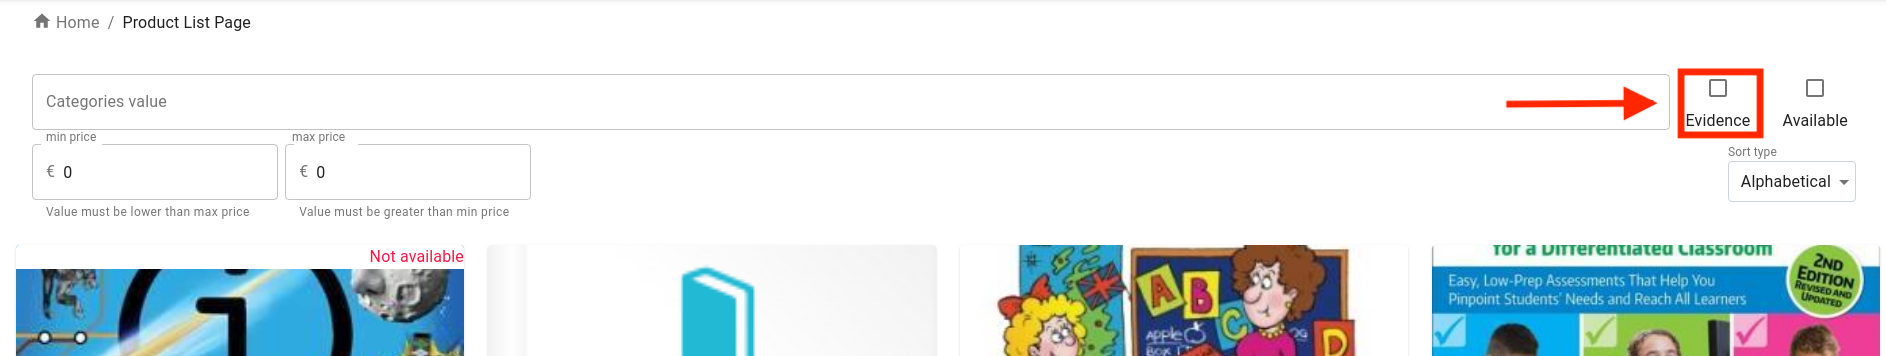
\includegraphics[scale=0.25]{Immagini/Venditore/plp.seller.png}
	\caption{Schermata prodotti con icona ricerca dei prodotti in evidenza}
	\label{fig:ProdottiEvidenza}
\end{figure}
\subsection{Gestione dei prodotti}
Il venditore può inserire, eliminare o modificare i prodotti all'interno della piattaforma.
\subsubsection{Aggiunta prodotto}
Per procedere con l'aggiunta di un nuovo prodotto, l'utente deve cliccare sull'icona (1) e verrà reindirizzato alla schermata per l'aggiunta di un prodotto.
\begin{figure}[H]
	\centering
	
\includegraphics[scale=0.4]{Immagini/Venditore/Seller Header.png}
	\caption{Barra del menù del venditore}
	\label{fig:BarraVenditore}
\end{figure}
\begin{figure}[H]
	\centering
	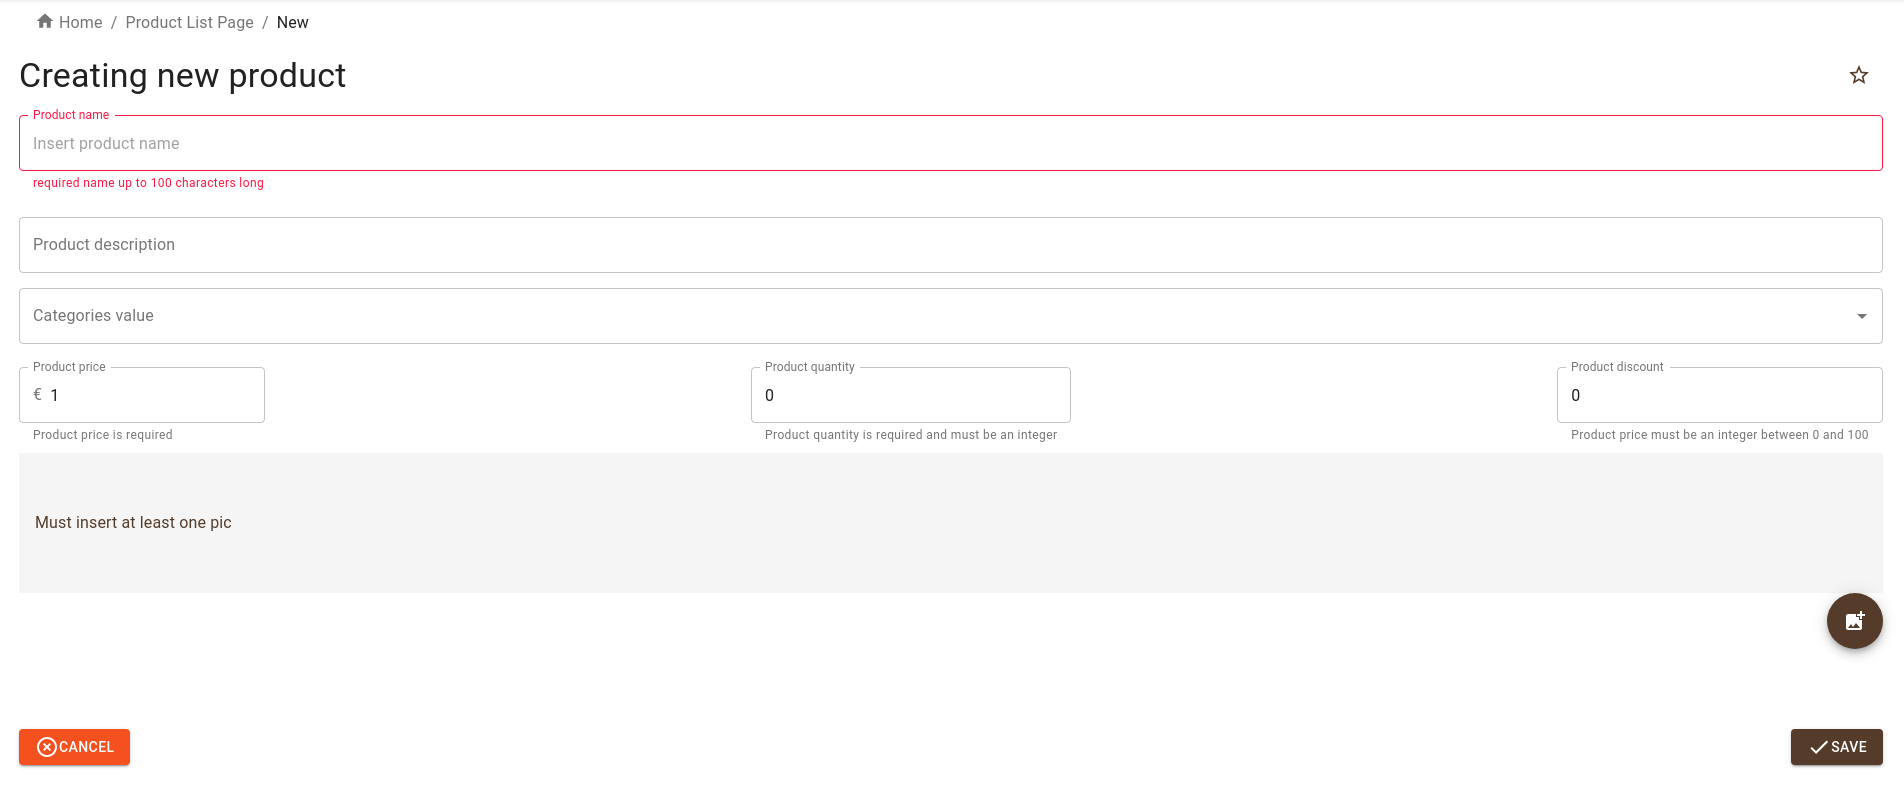
\includegraphics[scale=0.25]{Immagini/Venditore/pdp-new.seller.png}
	\caption{Aggiunta di un nuovo prodotto}
	\label{fig:AggiuntaProdotto}
\end{figure}
\subsubsection{Visualizzazione descrizione prodotto}
Il venditore può visualizzare la schermata di descrizione di un prodotto inserito e cliccando sulla icona a forma di stella posizionerà il prodotto tra quelli in evidenza.
\begin{figure}[H]
	\centering
	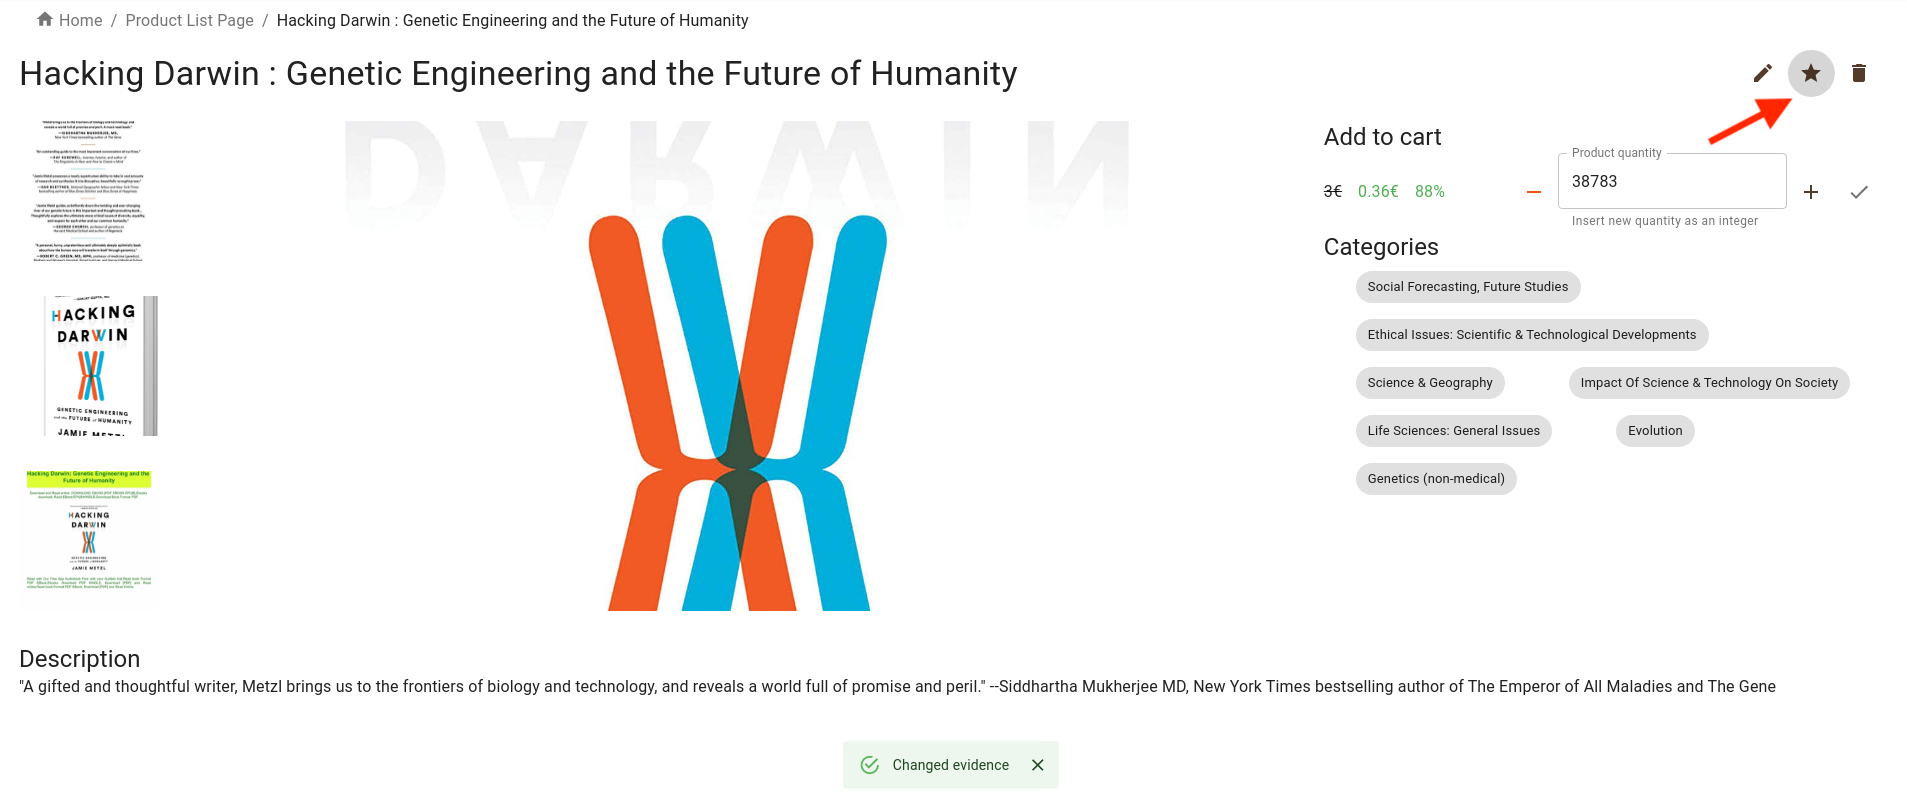
\includegraphics[scale=0.25]{Immagini/Venditore/pdp-evidence-setted.seller.png}
	\caption{Visualizzazione schermata di un prodotto in evidenza}
	\label{fig:VisualizzazioneProdotto}
\end{figure}
Per l'utente è inoltre possibile modificare la quantità disponibile del prodotto. 
\begin{figure}[H]
	\centering
	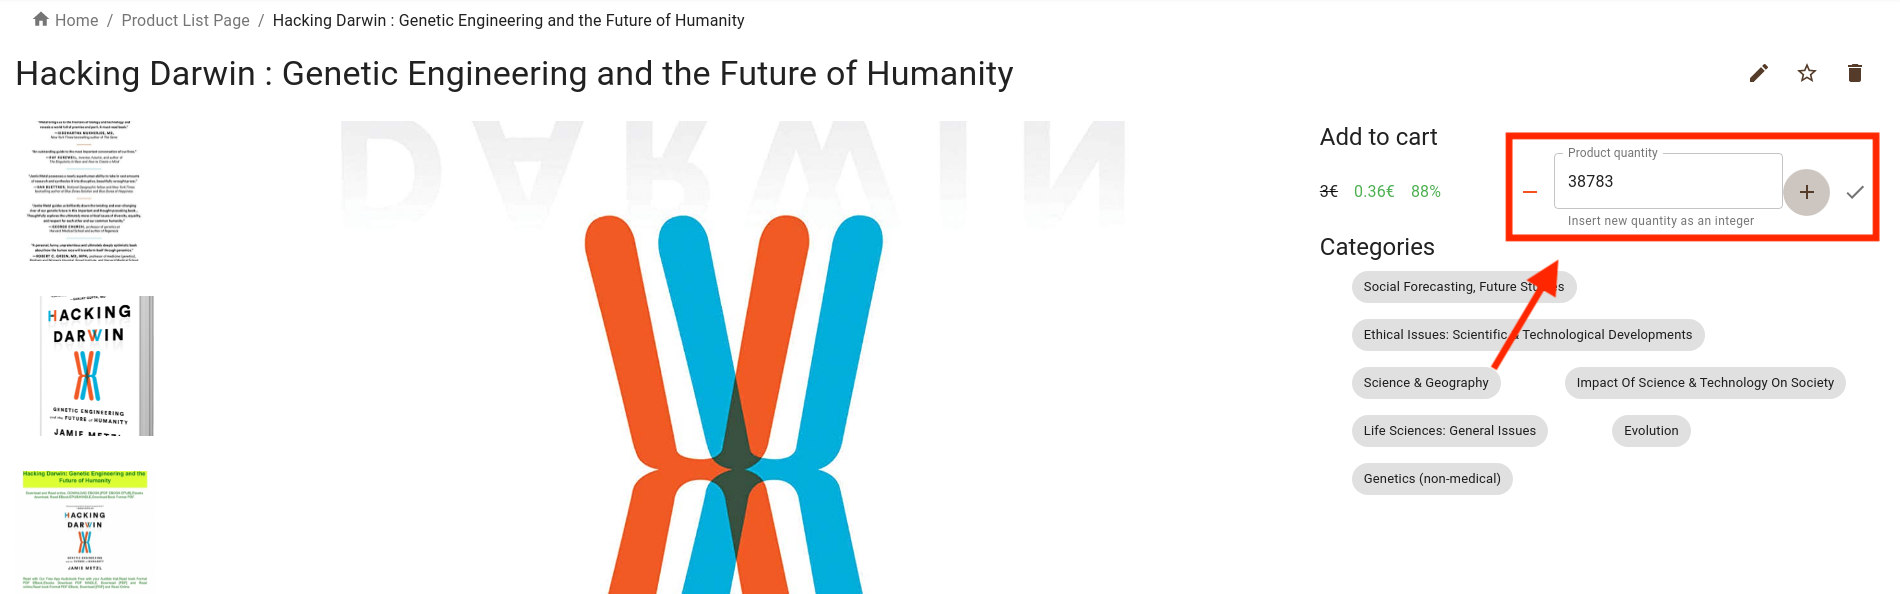
\includegraphics[scale=0.25]{Immagini/Venditore/pdp-changing-quantity.seller.png}
	\caption{Modifica quantità disponibile di un prodotto}
	\label{fig:QuantitàProdotto}
\end{figure}
\subsubsection{Eliminazione prodotto}
Per procedere con l'eliminazione di un prodotto, l'utente, dopo aver aperto la schermata di visualizzazione del prodotto che desidera eliminare, deve cliccare sull'icona del cestino e confermare la richiesta di eliminazione.
\begin{figure}[H]
	\centering
	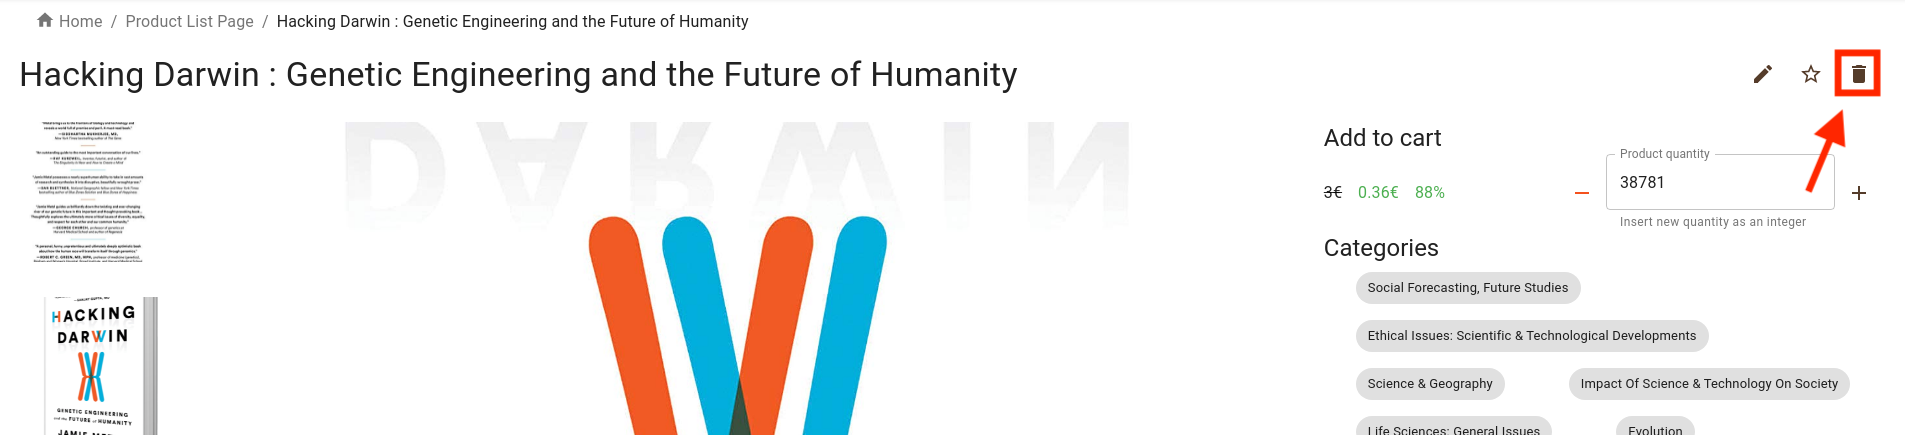
\includegraphics[scale=0.25]{Immagini/Venditore/pdp.sellerdelete.png}
	\caption{Pagina del prodotto con icona per l'eliminazione}
	\label{fig:EliminaP}
\end{figure}
\begin{figure}[H]
	\centering
	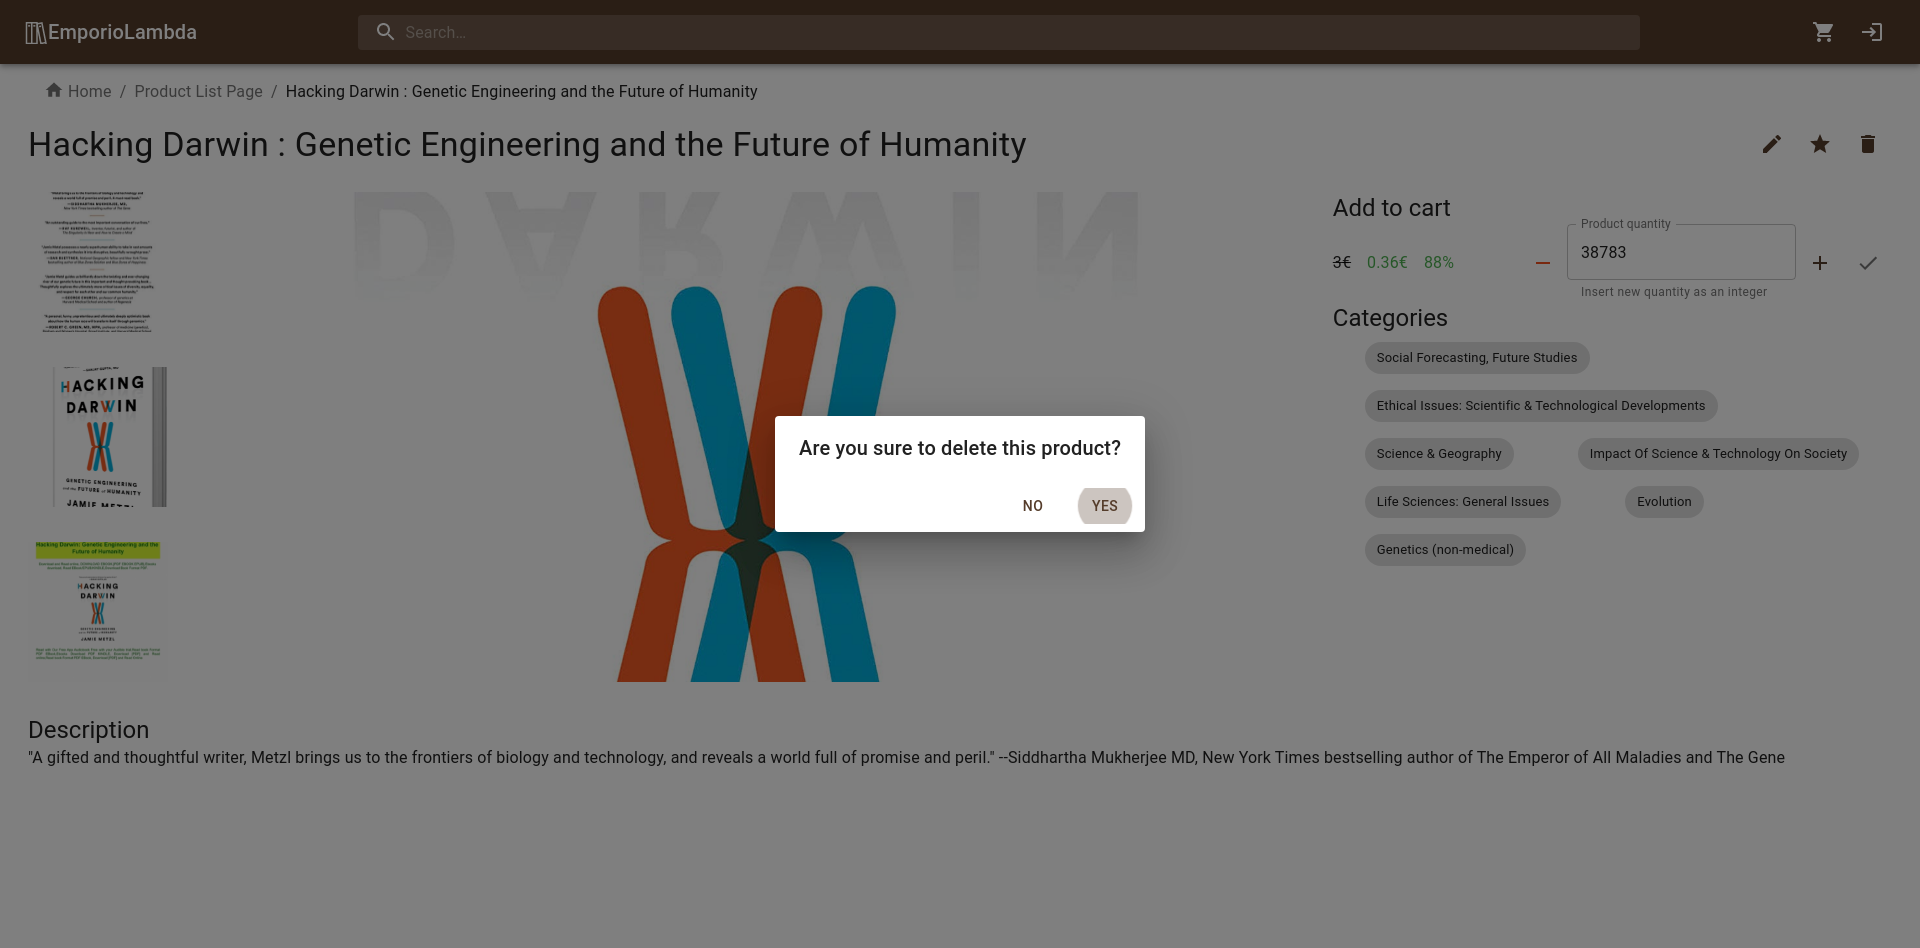
\includegraphics[scale=0.25]{Immagini/Venditore/pdp-remove.seller.png}
	\caption{Conferma eliminazione prodotto}
	\label{fig:EliminazioneProdotto}
\end{figure}
\subsubsection{Modifica prodotto}
Per procedere con la modifica di un prodotto, l'utente, dopo aver aperto la schermata di visualizzazione del prodotto che desidera eliminare, deve cliccare sull'icona del cestino e verrà reindirizzato alla pagina di modifica del prodotto.
\begin{figure}[H]
	\centering
	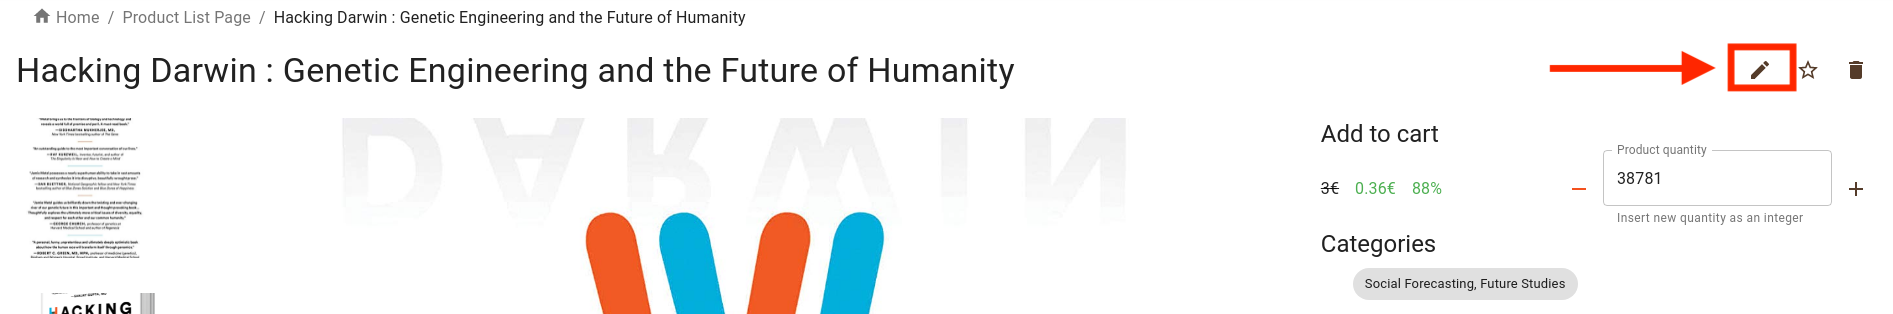
\includegraphics[scale=0.25]{Immagini/Venditore/pdp.sellermodify.png}
	\caption{Pagina del prodotto con icona per la modifica}
	\label{fig:ModificaP}
\end{figure}
\begin{figure}[H]
	\centering
	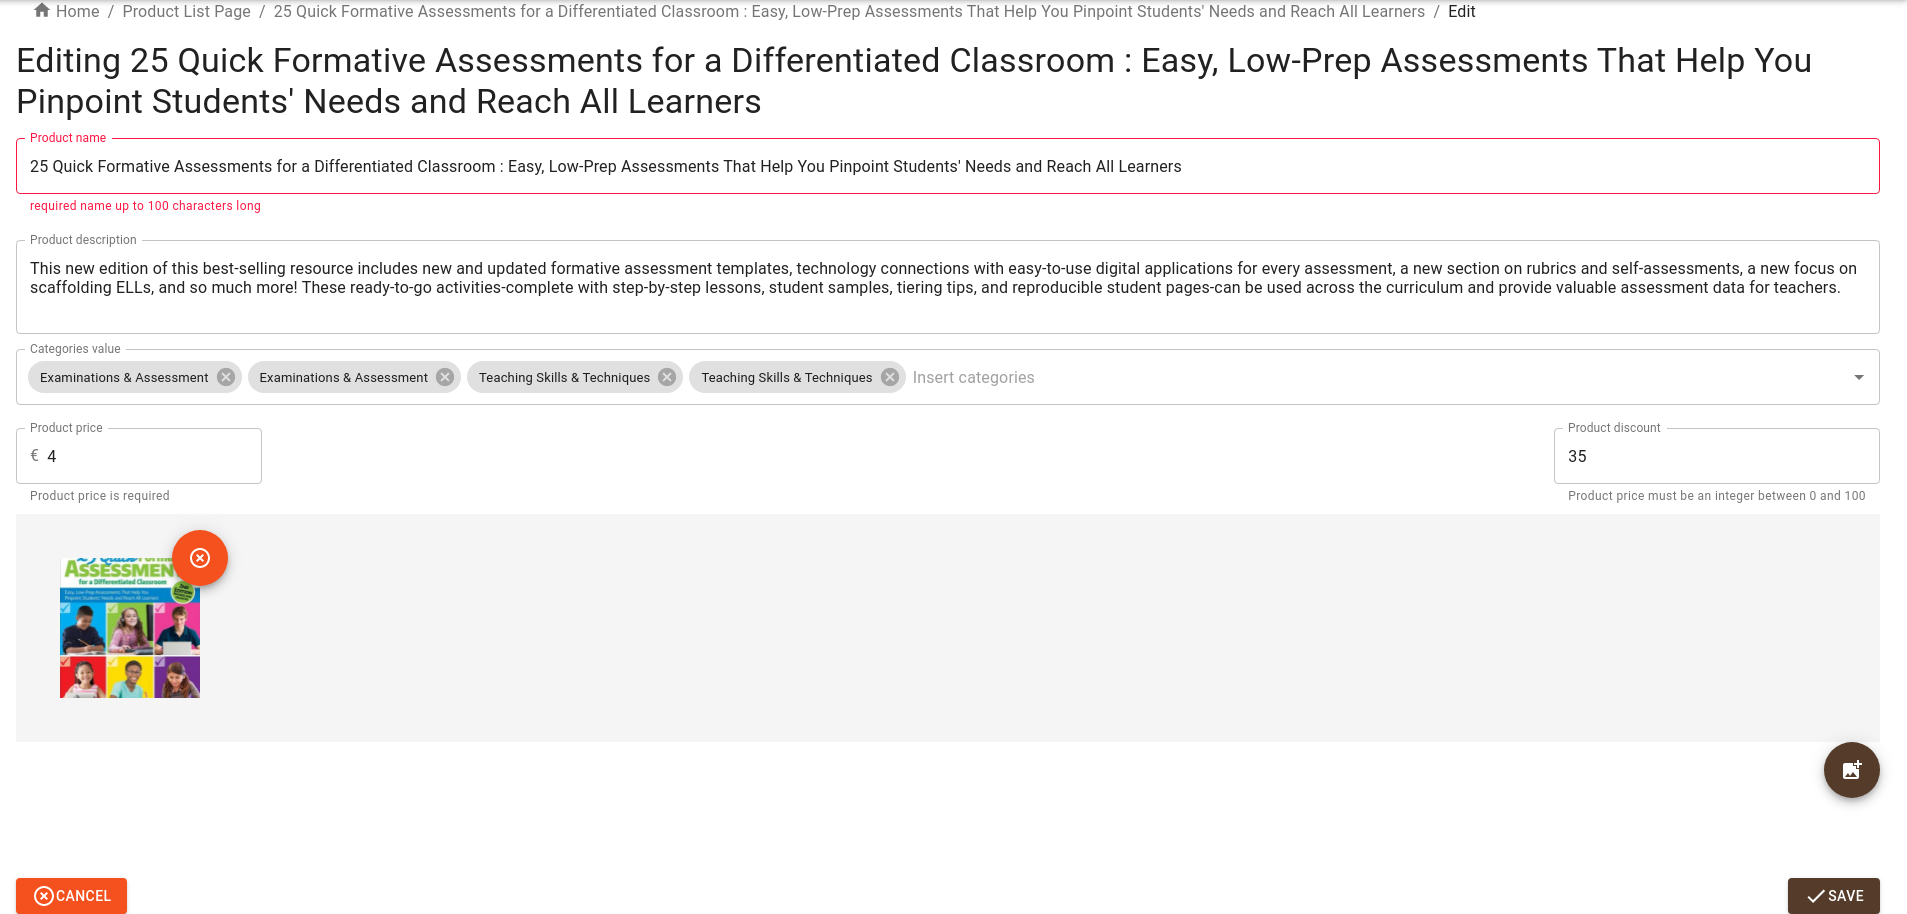
\includegraphics[scale=0.25]{Immagini/Venditore/pdp-edit.seller.png}
	\caption{Schermata di modifica prodotto}
	\label{fig:ModificaProdotto}
\end{figure}